%
% ======================================================================
\RequirePackage{docswitch}
% \flag is set by the user, through the makefile:
%    make note
%    make apj
% etc.
\setjournal{\flag}

\documentclass[\docopts]{\docclass}

% You could also define the document class directly
%\documentclass[]{emulateapj}

% Custom commands from LSST DESC, see texmf/styles/lsstdesc_macros.sty
\usepackage{lsstdesc_macros}

\usepackage{graphicx}
\graphicspath{{./}{./figures/}}
\bibliographystyle{apj}

% Add your own macros here:



%
% ======================================================================

\begin{document}

\title{ The LSST DESC Data Challenge 1: Generation and Analysis of Synthetic Images for Next Generation Surveys }

\maketitlepre

\begin{abstract}

The success of the Large Synoptic Survey Telescope (LSST) as a dark energy experiment will depend on controlling systematic effects for the various cosmological probes.  Simulations are critical for developing the methodology to estimate and mitigate these systematics.  In the first Data Challenge from the LSST Dark Energy Science Collaboration, we evaluate the potential systematic effects that will affect observables, with an emphasis on galaxy clustering.  We utilized two approaches to simulate LSST images, one of which involves fully realistic ray-tracing.  Simulated images were then processed, combined, and analyzed using the current version of the LSST Data Management pipeline.  Here we characterize the resulting systematics and implement corrections.  Our results demonstrate that we can generate realistic LSST-like simulated images and control the systematic effects, after processing these images, at a sufficient level to enable major advances in our knowledge of dark energy and cosmology. The methodology presented here can be easily translated to current and future imaging surveys.\CHECK{Rewrite?}
\end{abstract}

% Keywords are ignored in the LSST DESC Note style:
\dockeys{LSS , Data challenge, Systematics}

\maketitlepost

% ----------------------------------------------------------------------
%

\section{Introduction}
\label{sec:intro}

One of the most critical aspects in Stage IV experiments is the characterization of their instrumentation and systematic effects~\citep{2006astro.ph..9591A}. In the case of  LSST~\citep{Overview,ScienceBook,WhitePaper} this becomes especially difficult given its wide variety of cosmological probes. In this paper we present a methodology to characterize the LSST large-scale structure (LSS) transfer function and an analysis of potential systematic effects present in LSS analyses. \CHECK{rewrite}
% ---------------------------------------------------------------------

\section{DC1 data}
\label{sec:data}
In this paper we are going to analyze data from the LSST-DESC Data Challenge 1 (DC1)\CHECK{Add reference}. In particular, we are interested in the images from the DC1 dataset generated with a Fourier optics/analytic modeling using the \texttt{ImSim} package\footnote{\url{https://github.com/LSSTDESC/imSim}}, which internally calls the GalSim package~\citep{2015A&C....10..121R}  to generate the images for the different objects. The input catalog for these simulations is the CatSim\footnote{\url{https://www.lsst.org/scientists/simulations/catsim}} catalog. This catalog is based on the dark matter haloes from the Millenium simulation and a semi-analytic baryon model described in \citep{2006MNRAS.366..499D}. The galaxies are described as bulge+disk with no cosmic shear. This catalog covers a redshift range from $0 < z < 6$. The redshift and magnitude distribution can be seen at \figref{catalog_plots}. It has a higher number density of galaxies than the expected for LSST, since it contains sources fainter than its detectable limits. This simulation also contains stars represented as point sources and drawn from the Galfast model~\citep{2008ApJ...673..864J} with peculiar motion. CatSim also contains associates each source with an SED.

\begin{figure}
\centering
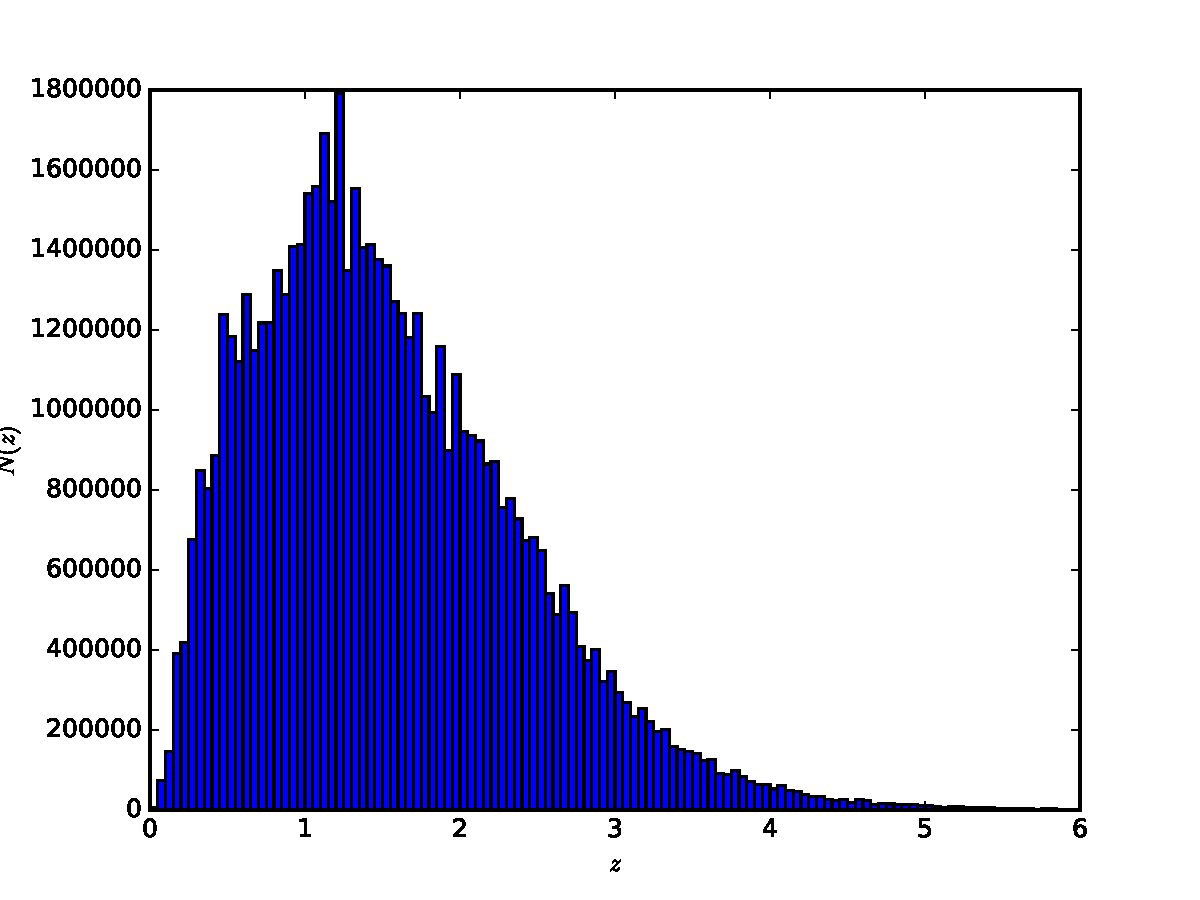
\includegraphics[width=0.9\columnwidth]{n_z_galaxies.pdf}
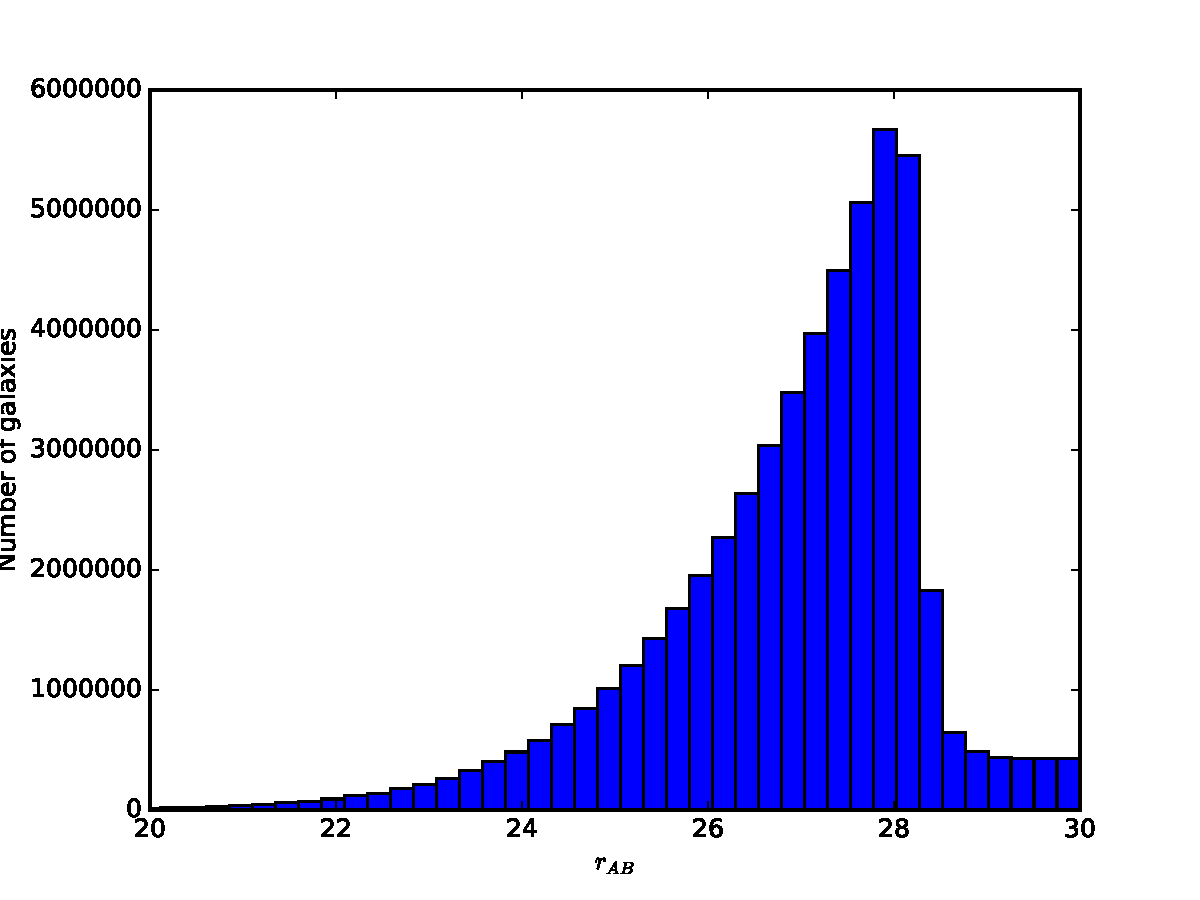
\includegraphics[width=0.9\columnwidth]{n_m_galaxies.pdf}
\caption{Redshift (top) and magnitude (bottom) distribution for the galaxies used as inputs for DC1.}
\label{fig:catalog_plots}
\end{figure}

In total the input catalog contains approximately $63.1$ million sources of which, $61.3$ million are galaxies and $1.8$ million are stars. Using this catalog we generate images covering an area of approximately $40$ square degrees ($4$ pointings) in r-band to LSST full depth ($10$ years). The final footprint can be seen in \figref{footprint}

\begin{figure}
\centering
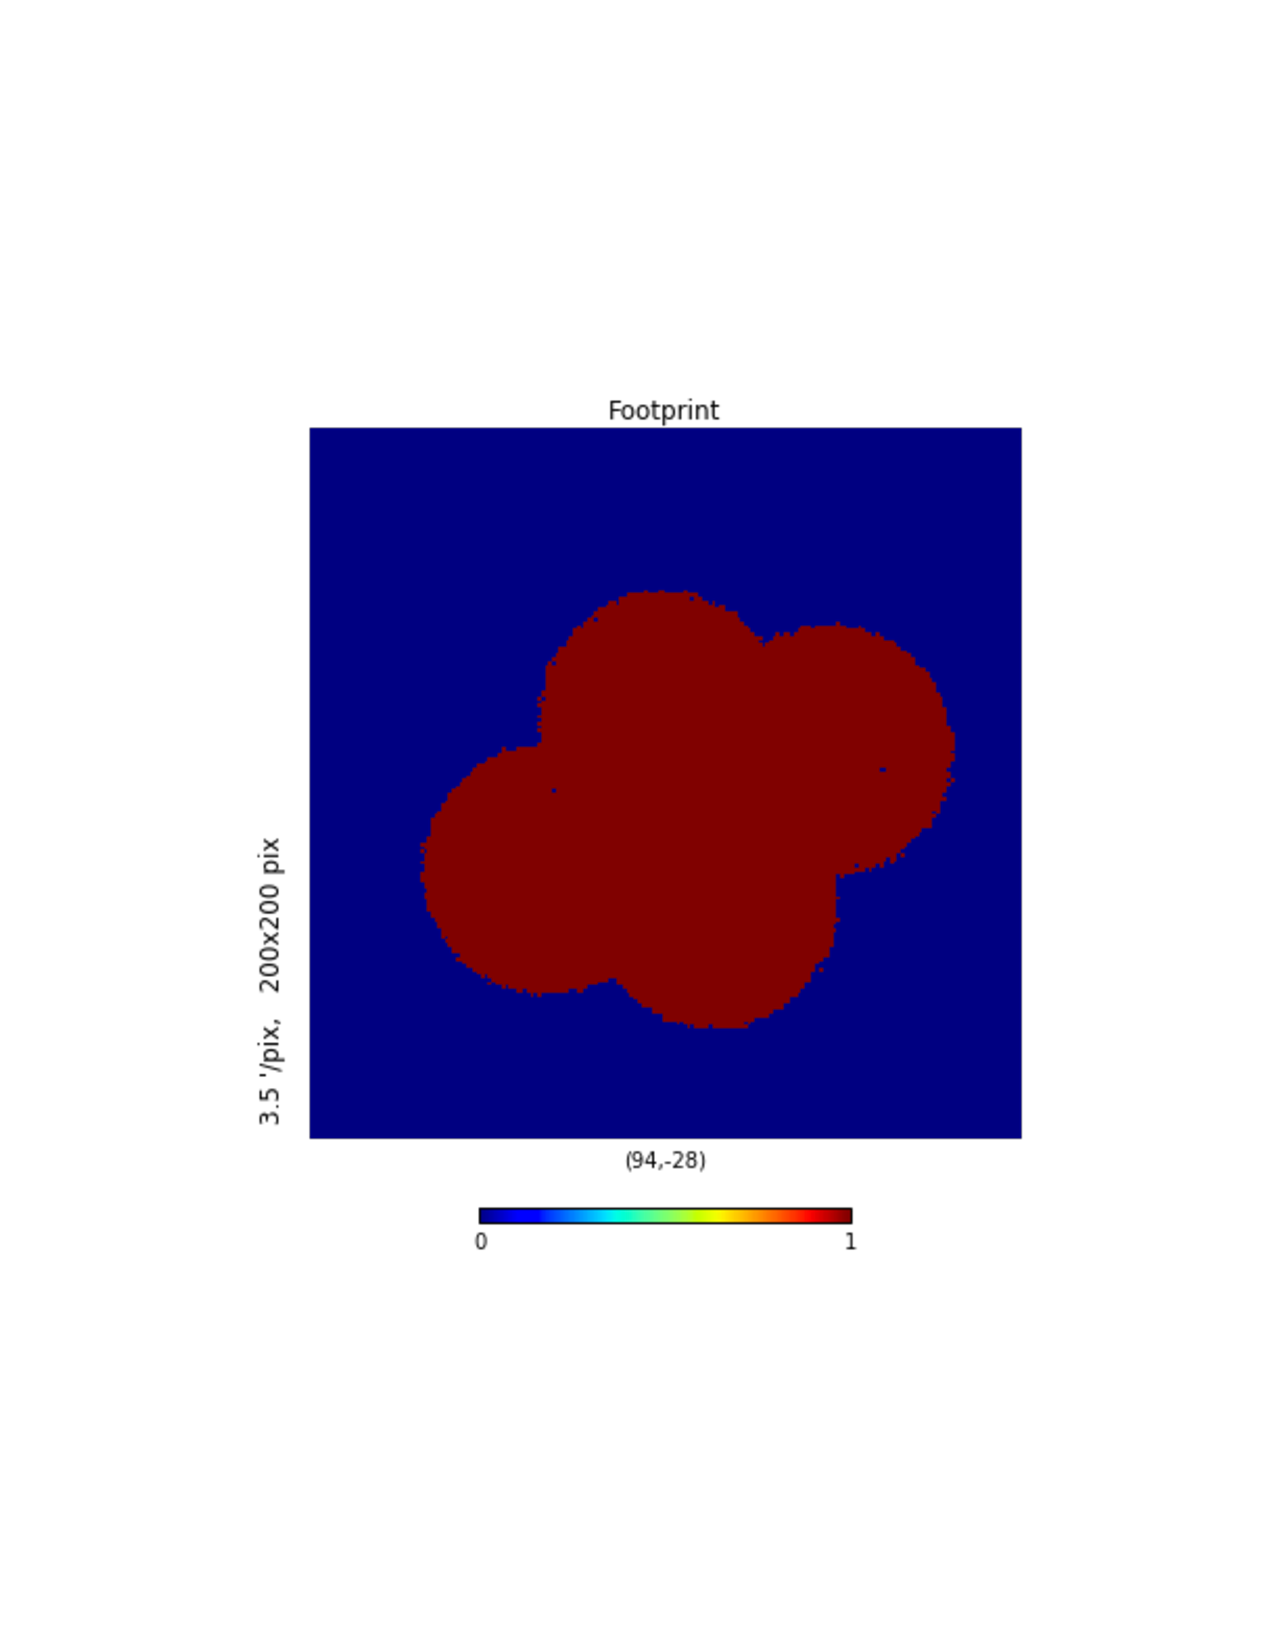
\includegraphics[trim={4cm, 6cm, 4cm, 6cm},clip,width=0.9\columnwidth]{footprint.pdf}
\caption{Footprint of the DC1 dataset. We simulate 4 LSST full focal plane pointings which roughly corresponds to 40 square degrees.}
\label{fig:footprint}
\end{figure}

Two sets of images were generated using \texttt{imSim}: One with no dithering, which we will refer to \textit{undithered}; and the other one which includes the dithering strategy in the \texttt{minion\_1016\_new\_dithers} OpSim\footnote{\url{https://www.lsst.org/scientists/simulations/opsim}} database presented in ref.~\citep{2016ApJ...829...50A}. We will refer to the latter dataset as the \textit{dithered} run. We do not simulate images out of the footprint in \figref{footprint}. Using these two datasets allows us to make a fair comparison between them, and see the advantages and disadvantages of each approach.

The outputs of these simulations are then processed using the LSST data management (DM) stack~\citep{Overview,ScienceBook,WhitePaper,2017arXiv170506766B}  \CHECK{Is there any other reference for the stack?}. The DM stack is intended to be the software used to process the data produced by LSST. Although it is still under development, most of the pieces are already meeting the science requirements or very close to do that. Running the DM stack on this dataset also constitutes a necessary test for this invaluable piece of LSST. The stack can be divided into three main steps: the coadding step where the images are put together to form a deeper image than each individual exposure; the detection step, where the coadded image is analyzed searching for peaks on the counts; and the measurement step, where these peaks are characterized. The DM stack performs these three steps automatically and provides calibrated images and a source catalog with $\sim 10.6$ million objects with position, flux and shape information.

An example of a coadd image can be seen at \figref{coadd_example}.

\begin{figure}
\centering
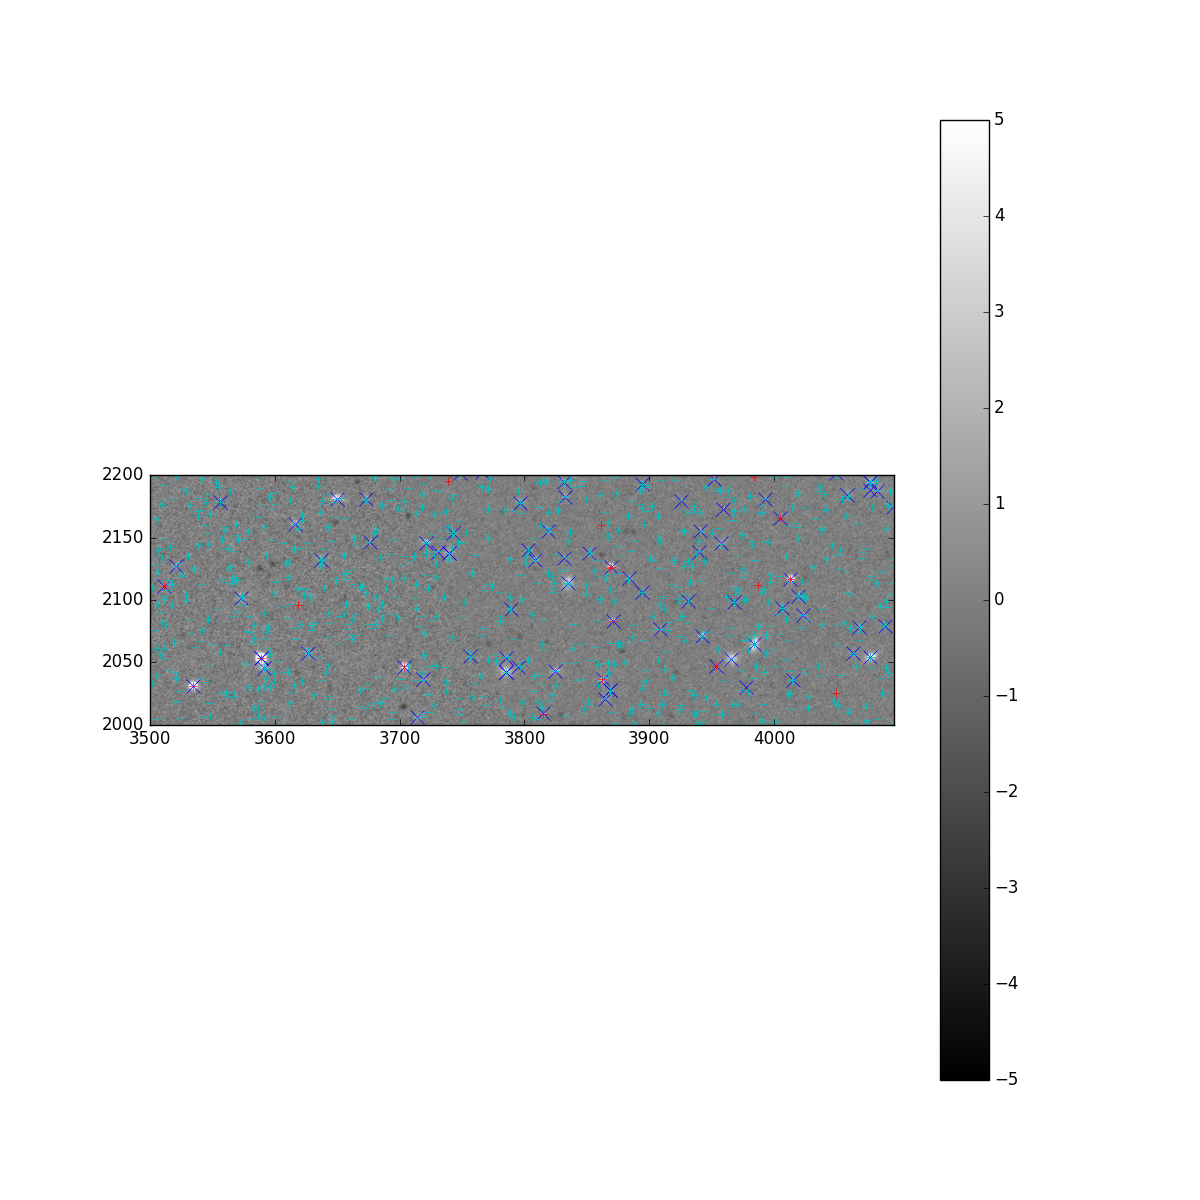
\includegraphics[trim={3cm, 14cm, 12cm, 12cm},clip,width=0.9\columnwidth]{field.png}
\caption{Example of a 550 $\times$ 200 pixel simulated field. The axes show the pixel number in the CCD. The input galaxies are marked with cyan $+$, the input stars are marked with red $+$, and the detected sources are marked with blue $\times$. We can appreciate the vast difference in density between the simulation and the output given that CatSim contains objects fainter than what LSST can detect.}
\label{fig:coadd_example}
\end{figure}

% ----------------------------------------------------------------------

\section{Generating depth maps}
\label{sec:masking}

In order to estimate the depth in the coadd catalogs we select the stars by using \texttt{base\_ClassificationExtendedness\_value==0}. This ensures selecting
PSF-like objects. After this, we have two different approaches:

\begin{enumerate}
\item In the first approach we generate a HEALPix~\citep{2005ApJ...622..759G} map containing the PSF-like objects detected with a signal-to-noise ratio (SNR) higher or equal than 5 (\texttt{base\_PsfFlux\_flux/base\_PsfFlux\_fluxSigma>=5}), and we assign to each pixel the value of the
dimmest object contained in it.
\item The second procedure also generates a HEALPix~\citep{2005ApJ...622..759G} map containing the PSF-like objects. Then in each pixel, we compute the median SNR as a function of the magnitude and get the magnitude at which SNR is the closest to 5.
\end{enumerate}

These two procedures yield very similar results (within $\sim 4\%$) as it can be seen in \figref{depth_comparison}. We checked that the maps built selecting galaxies instead of stars are compatible as well. We will select our footprint according to the depth map using the second methodology which can be seen in \figref{depth_maps}.

\begin{figure}
\centering
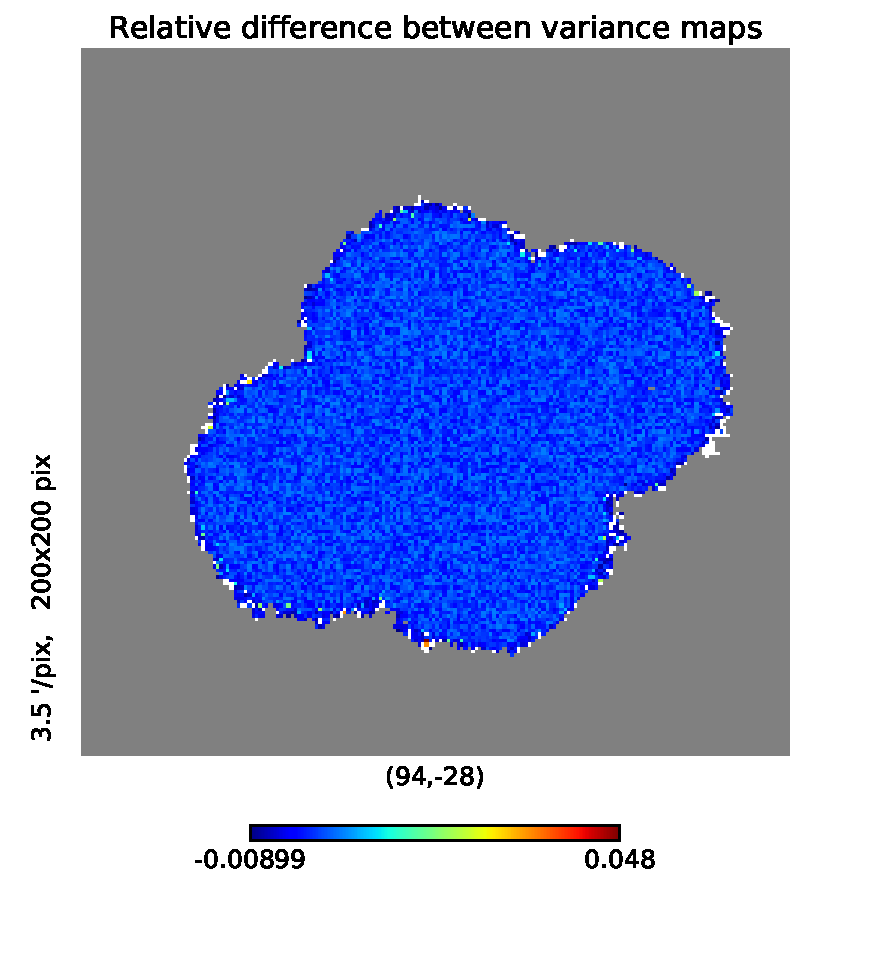
\includegraphics[width=0.9\columnwidth]{imsim_dithered_depth_difference.pdf}
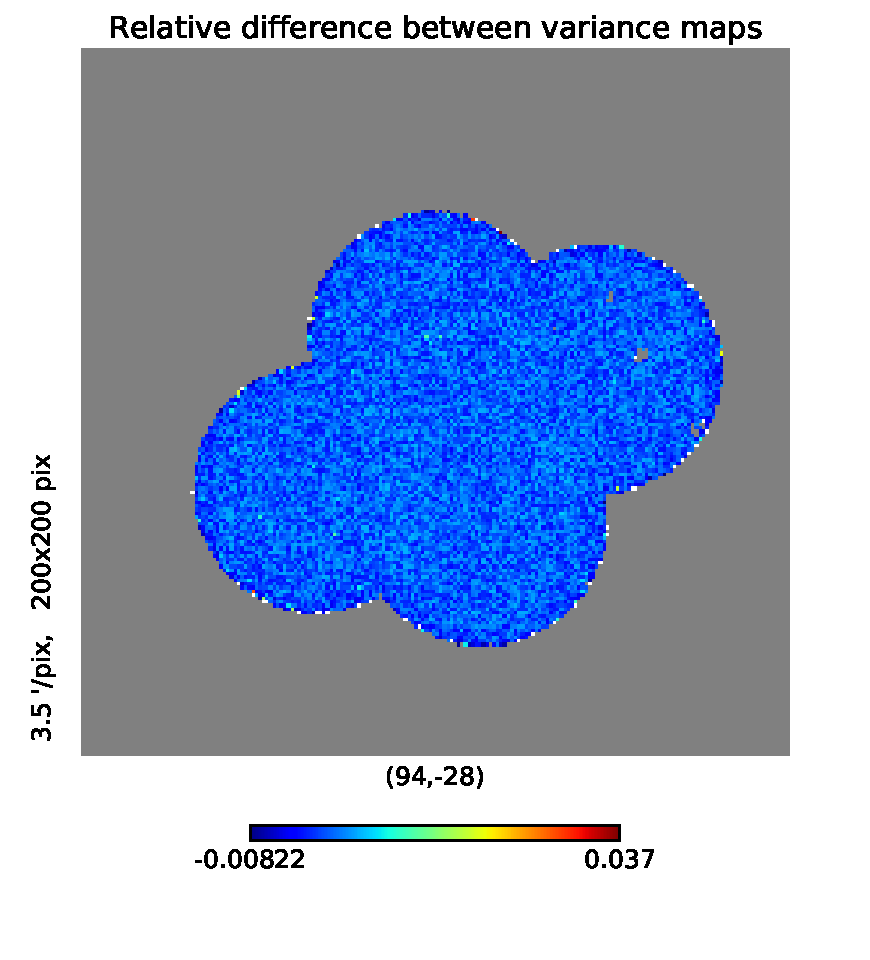
\includegraphics[width=0.9\columnwidth]{imsim_undithered_depth_difference.pdf}
\caption{Relative difference between the depth calculated using the two methods presented in the text for the dithered (top) and undithered (bottom) fields.}
\label{fig:depth_comparison}
\end{figure}

\begin{figure}
\centering
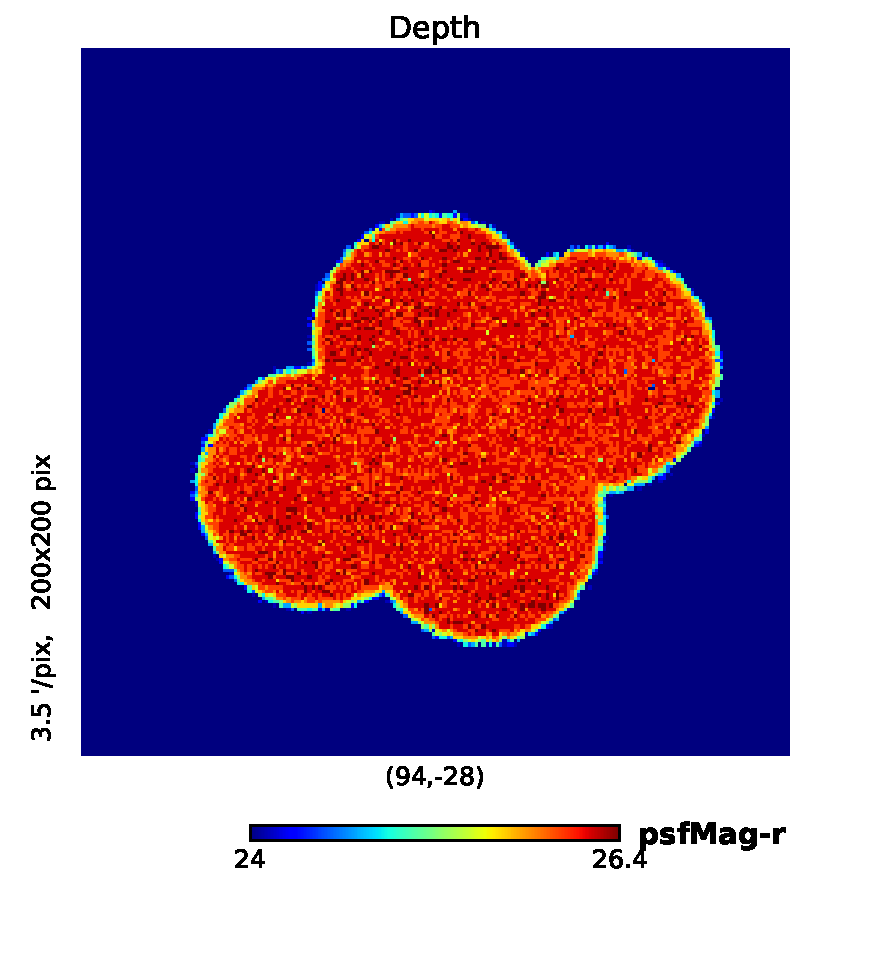
\includegraphics[width=0.9\columnwidth]{imsim_dithered_depth_snr_stars.pdf}
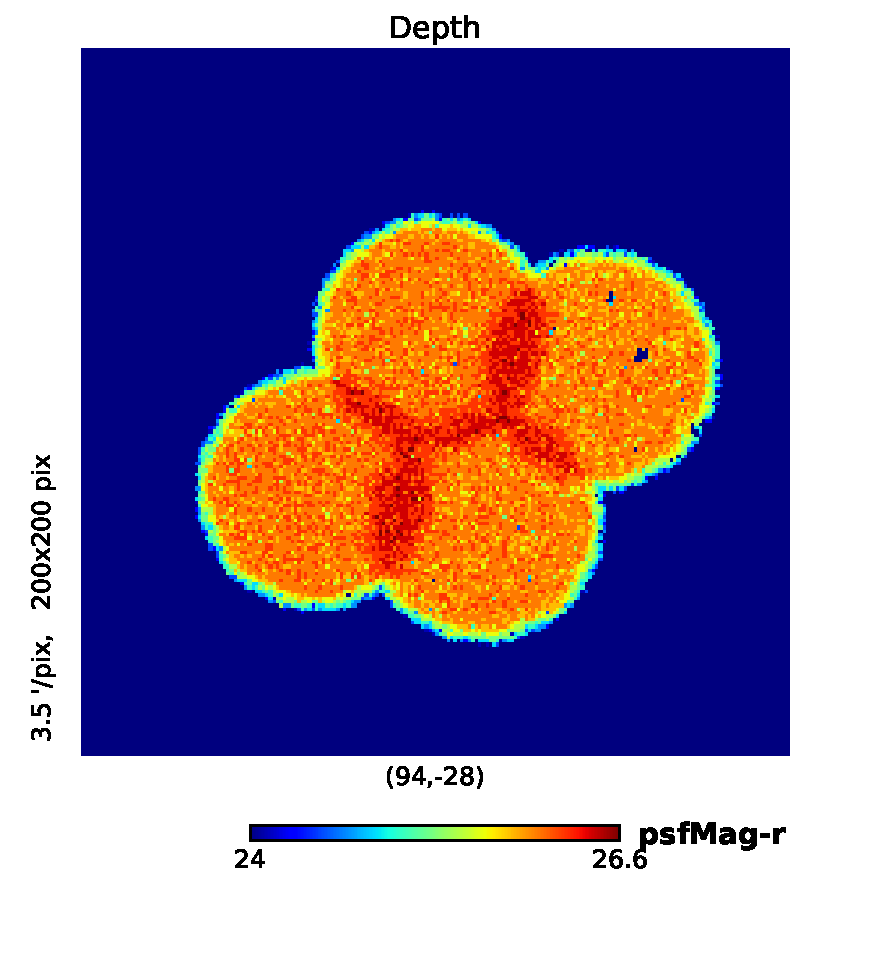
\includegraphics[width=0.9\columnwidth]{imsim_undithered_depth_snr_stars.pdf}
\caption{5-$\sigma$ depth for the dithered (top) and undithered (bottom) fields.}
\label{fig:depth_maps}
\end{figure}

\subsection{Bright objects masking and data selection}

Bright objects produce significant effects in the image that affects the detection and measurement of neighboring objects. Some examples of the effect of these objects are: saturation of the CCD, large diffraction spikes, obscuration of neighboring sources, etc. Thus, masking a region around these sources makes a more complicated footprint but largely simplifies the analysis of systematic effects. In order to evaluate the effect of this sources, we use the stars from the input catalog, we divide them in different magnitude bins, and we count the detected objects in a given radius. However, the number of objects in a given radius is dependent of the number of stars in each bin and subject to statistical fluctuations. Therefore, we use instead the average on this number for the different magnitude bins. This analysis is largely simplified if we use the numerical derivative of this quantity. In \figref{galdens_derivative} we can see that there is an excess of sources at distances lower than 10 arcseconds for the brightest stars. This is mainly due to the existence of fake sources around these bright objects. The brighter sources also have a larger noise, the DM deblender models the brightest source and subtracts this model looking for fainter sources that can be blended together with it. However, sometimes there are large noise peaks that have not been subtracted. These large noise peaks are detected in later stages as individual (point-like) sources giving as a result these fake sources. However, we do not see any obscuration present at the scales that we are interested (1 arcmin and higher) so it seems that no masking is required but we need to select the objects for our analysis carefully.

\begin{figure}
\centering
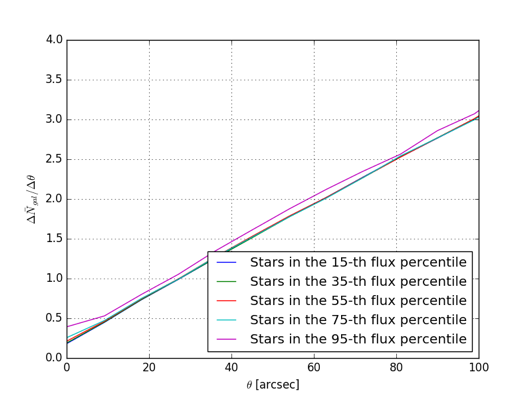
\includegraphics[width=0.9\columnwidth]{dngal_dtheta.png}
\caption{Mean increment in the number of detected objects around stars in the 95th flux percentile (magenta), the 75th percentile (cyan), the 55th percentile (red), the 35th percentile (green) and the 15th percentile (blue). We see that for the brightest percentiles there is no obscuration present but a overdensity of targets. These are mainly noise peaks identified as point sources.}
\label{fig:galdens_derivative}
\end{figure}

We checked the detection efficiency of galaxies in our sample. In order to do so we selected galaxies in the catalog using the variable \texttt{base\_ClassificationExtendedness\_value} as a star/galaxy separator as in ref.~\citep{2017arXiv170506766B}. Objects where this variable is 1 are more likely to be galaxies, whereas the objects where it is 0 are more likely to be stars. We also made some quality cuts by selecting the objects with \texttt{detect\_isPrimary==True}. This ensures that the object has been fully deblended and that the detection was not close to the edge of a coadded image. The results can be seen in \figref{completeness} where we computed the ratio o of detected objects classified as galaxies and the input number of galaxies, $\varepsilon$ as a function of magnitude. We checked this ratio for both the dithered and undithered catalogs and in pixels where the depths were higher than 25.7 and 26.25. We used \texttt{CMODEL\_MAG} (see ref.~\citep{2017arXiv170506766B} for more details) as the reference magnitude for the detected objects and the true magnitude for the input galaxies.

\begin{figure}
\centering
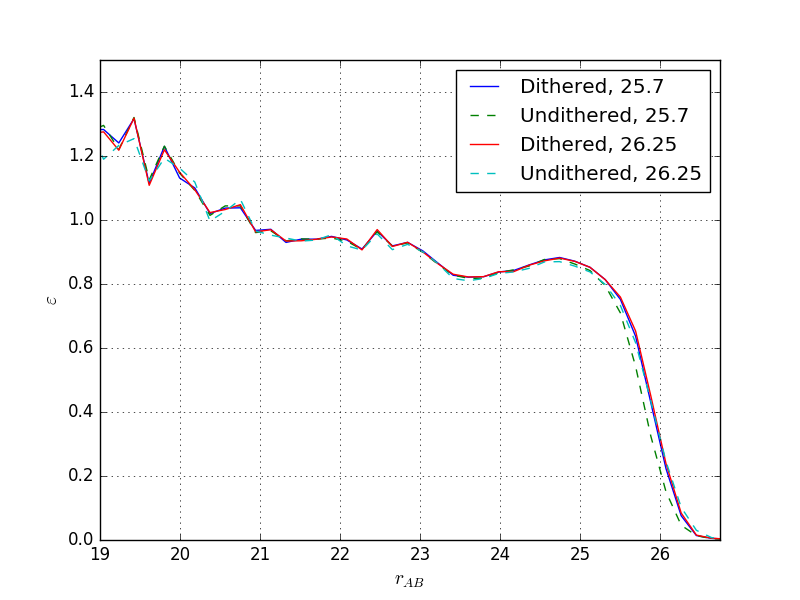
\includegraphics[width=0.9\columnwidth]{completeness.png}
\caption{Number of detected objects classified as galaxies divided by the number input galaxies as a function of magnitude. We see that the detection efficiency is larger than 80\% for the most part and a considerable fraction of objects with magnitude lower than 20 are being misclassified.}
\label{fig:completeness}
\end{figure}

Looking at \figref{completeness} it seems that selecting galaxies with \texttt{base\_ClassificationExtendedness\_value==1}, \texttt{detect\_isPrimary==True} and \texttt{CMODEL\_MAG $>$ 21} is enough to get rid of most potential problems with fake detections. On top of that, it seems that selecting \texttt{CMODEL\_MAG $<$ 25.3} ensures good level of completeness ($\sim 80\%$). Uniformity is ensured by selecting the galaxies that lie within HEALPixels where the depth is greater or equal than 25.3. After these selection cuts we end up with 4.4 million galaxies for the dithered field and 4.3 for the undithered field. 
% ----------------------------------------------------------------------

\section{Clustering results}
\label{sec:results}

\CHECK{Add something as intro for this section}. In this section we analyze the two point clustering statistics for both the dithered and undithered catalogs in real and harmonic space and check the consistency between the input and measured observables. 

\subsection{2-point correlation function}
Using the samples presented in previous sections, we measure the 2-point correlation function using the package \texttt{TreeCorr}~\citep{2004MNRAS.352..338J} with the Landy \& Szalay estimator~\citep{1993ApJ...412...64L}.

\begin{equation}
w(\theta) = \frac{DD - 2 DR + RR}{RR}
\end{equation} 
where $DD, DR$, and $RR$ are the number of pairs of objects taking from the data $D$ or the random catalog $R$ that covers the footprint. We use 15 angular log-spaced bins between $\theta=0.05^{\circ}$ and $\theta=10^{\circ}$. The number of bins has been chosen so that the resulting covariance matrix is nearly diagonal. The covariance matrices are calculated using the delete-one jackknife technique~\citep{Shao:1986:DJB,2009MNRAS.396...19N}. We divide the footprint in $N_{JK}=100$ regions. These regions are defined using the K-means algorithm from the package \texttt{kmeans\_radec}\footnote{\url{https://github.com/esheldon/kmeans\_radec}}. The covariance matrix is then computed as
\begin{equation}
\mathrm{Cov}_{JK}(\theta_{i},\theta_{j})=\frac{N_{JK}-1}{N_{JK}}\sum_{k=1}^{N_{JK}}\Delta w_{k}(\theta_{i}) \Delta w_{k}(\theta_{j})
\end{equation}
\begin{equation}
\Delta w_{k}(\theta_{i}) = w_{k}(\theta_{i})-\bar{w}(\theta_{i})
\end{equation}
Where $w_{k}(\theta_{i})$ is the value of the correlation function when deleting the $k$-th region at the scale $\theta_{i}$, and $\bar{w}(\theta_{i})$ is the average correlation function at that same scale. We compute the correlation function on the dithered and undithered catalogs using their respective footprints, and we compare with the truth catalog in the dithered footprint using the same magnitude cuts. The results can be seen at \figref{2pt_corr}. 

We also show the correlation matrix,
\begin{equation}
\mathrm{Corr}_{ij}=\frac{\mathrm{Cov}_{ij}}{\sqrt{\mathrm{Cov}_{ii}\mathrm{Cov}_{jj}}}
\end{equation}
in \figref{2pt_cov} where we can see that in both cases the matrices are almost diagonal.
\begin{figure}
\centering
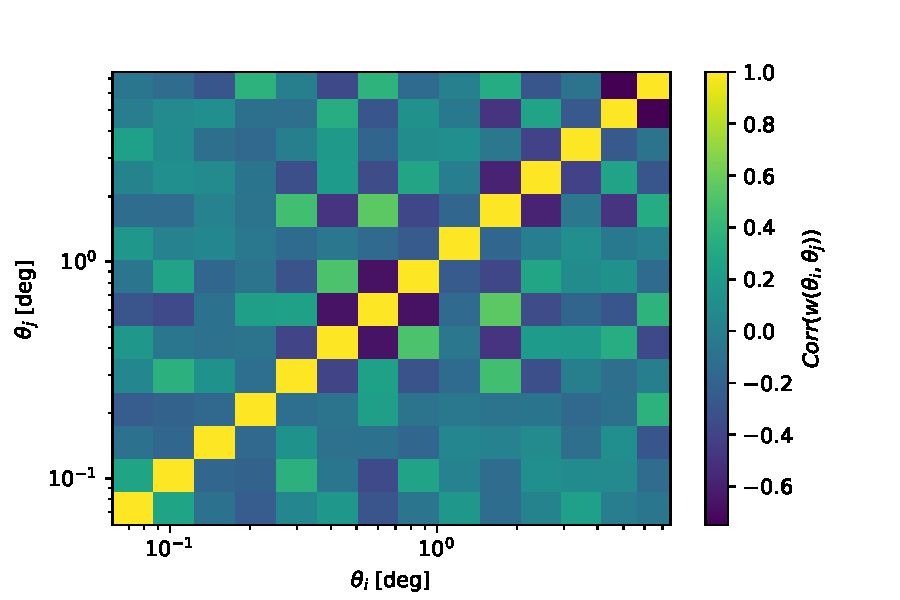
\includegraphics[width=0.9\columnwidth]{correlation_matrix_dithered_25p3.pdf}
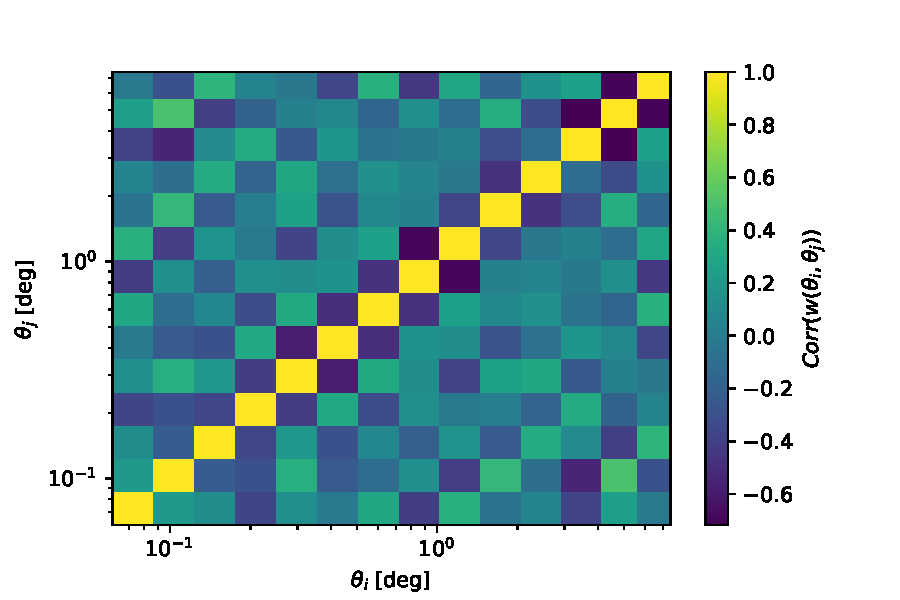
\includegraphics[width=0.9\columnwidth]{correlation_matrix_undithered_25p3.pdf}
\caption{Correlation matrices for the dithered (top) and undithered catalogs (bottom).}
\label{fig:2pt_cov}
\end{figure}
\subsection{Angular power spectrum}
We measure the angular power spectrum using the \texttt{NaMaster}\footnote{\url{https://github.com/damonge/NaMaster}} package. This package computes the cross-power-spectra of masked fields with an arbitrary number of contaminants using a pseudo-$C_{\ell}$ approach~\citep{2002ApJ...567....2H,2017MNRAS.465.1847E}. As we do for real space, we select the number of $\ell$ bins so that the covariance matrix is almost diagonal. In this case we calculate the power spectrum in the range $0 < \ell < 2000$ and $\Delta \ell = 75$. We calculate the covariance matrices with two different approaches: One consists in the same delete-one jackknife technique performed in real space; in the other approach we compute the Gaussian covariances~\citep{Dodelson:1282338,2007MNRAS.381.1347C}
\begin{equation}
\mathrm{Cov}_{\ell\ell'}=\frac{2}{f_{sky}}\left(\frac{C_{\ell}^{2}}{2\ell+1}+\frac{1}{\bar{n}^{2}}\right)\delta_{\ell\ell'}
\end{equation}
where $\bar{n}$ is the number density (objects per steradian). We compute the theoretical prediction for the power-spectra with \texttt{CCL}\footnote{\url{https://github.com/LSSTDESC/CCL}} and use them to calculate the covariance matrices given that the predictions are noise-free.
\begin{equation}
C_{\ell}^{TH} = \frac{2}{\pi}\int{dz} \left(\frac{dn(z)}{dz}\right)^{2} b^{2}(z) \int{dk k^{2} P(k,z)j^{2}_{\ell}(kr(z))}
\end{equation}
Where $P(k,z)$ is the power spectrum, $b(z)$ is the bias and $\frac{dn}{dz}$ is the number density as a function of redshift. We use the Millenium cosmological parameters~\citep{2005Nature.435.629S} ($\Omega_{m}=0.25$,$\Omega_{b}=0.045$,$\Omega_{\Lambda}=0.75$, $n=1$, $\sigma_{8}=0.9$, $h=0.73$), and the $\frac{dn}{dz}$ built with the input catalog using the same magnitude cuts. The results can be seen in \figref{power_spectra}. It seems that there is a small bias between the measured power-spectra and the input data power-spectrum (and between the dithered and undithered data), however, the error bars in the data are large enough to make this bias negligible.
\begin{figure}
\centering
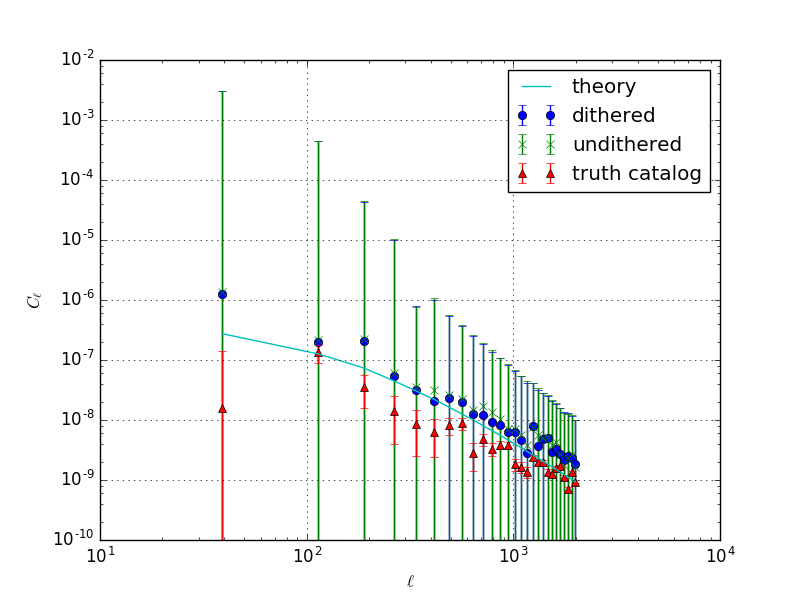
\includegraphics[width=0.9\columnwidth]{results_Cl_25p3.png}
\caption{Measured power spectra for the input (red), undithered (green) and dithered (blue) datasets with \texttt{NaMaster}. The error bars are computed using the Gaussian approximation. All datasets seem to be compatible with the theoretical prediction (cyan) within 1-$\sigma$.}
\label{fig:power_spectra}
\end{figure}
\subsection{Systematic effects}
In this section we analyze the different systematic effects affecting the DC1 data. We will consider the following observational quantities as sources for systematic uncertainties:
\begin{itemize}
\item Extinction: The CatSim catalog provides the value for the magnitudes already corrected for extinction using the SFD map~\citep{1998ApJ...500..525S}. We use this map to cross-correlate with our galaxy catalogs.
\item Stellar contamination: In this case we just build a HEALPix map using the input CatSim stellar catalog to cross-correlate with our galaxy catalogs.
\item Sky-background: We use the observed background level in each exposure and assign that value to the HEALPixel with $N_{side}=2048$ that corresponds to the pointing position. After this we calculate the median value in each HEALPixel and use them to compute the cross-correlations with the galaxy catalogs. The caveat of this approach is that we are not propagating the geometry of the focal plane.
\item Sky-noise: We use the observed noise background level in each exposure and proceed as in the previous case to build a HEALPix map with which we will cross-correlate.
\item Seeing: We proceed as before and use the observed seeing in each exposure and build a HEALPix map.
\end{itemize}
These maps are shown in \figref{systematic_maps} and \figref{systematic_maps2}. 

In the case of the real space measurements, we proceed the same way as ref.~\citep{2016MNRAS.455.4301C} to compute the impact of the different potential sources for systematic uncertainty. We compute the auto and cross-correlations of these maps and our data samples to obtain the ``true`` correlation function and since the cross-correlations between different systematic maps are negligible (\textit{i.e.} they are independent) we can write,
\begin{equation}
w(\theta)_{true} =w(\theta)_{obs} -  \sum_{sys}  \frac{{w}^{2}_{sys,cross}}{w_{sys,auto}}
\end{equation}
where we sum over all relevant systematics, $w_{sys,cross}$ is the cross-correlation between the considered map and the observed data, and $w_{sys,auto}$ is the auto-correlation of the considered maps. For the stellar contamination we also follow the procedure presented in ref.~\citep{2016MNRAS.455.4301C}. Given a stellar fraction $f_{star}$ the ``true`` galaxy correlation function is given by
\begin{equation}
w_{gal} = \left(1+f_{star}\right)^{2}\left(w_{obs} - f_{star}^{2}w_{sg} - \frac{f_{star}^{4}}{\left(1+f_{star}\right)^{2}}\right)
\end{equation}
where $w_{sg}$ is the cross-correlation between our stellar map and the observed galaxies.

Comparing with the input catalog we select those objects classified as galaxies whose centroids lie within 2 pixels of a star from the input catalog. From those, we select the objects that have a magnitude difference smaller than 30 mmags. Doing this we estimate a stellar contamination of $f_{star}=7.2\%$ in our sample.

We compare the correction term for the different systematics to the measured signal obtaining the results in \figref{sys_realspace}, where we can appreciate that the dithering strategy is working reducing the impact of the systematics, keeping them under control and at percent level for this ``small`` area, improving the signal-to-noise in addition to other benefits explored in ref.~\citep{2016ApJ...829...50A}. This is also seen \figref{2pt_corr} where we clearly see that the uncorrected and corrected correlation function for the dithered field are essentially the same.
\begin{figure}
\centering
%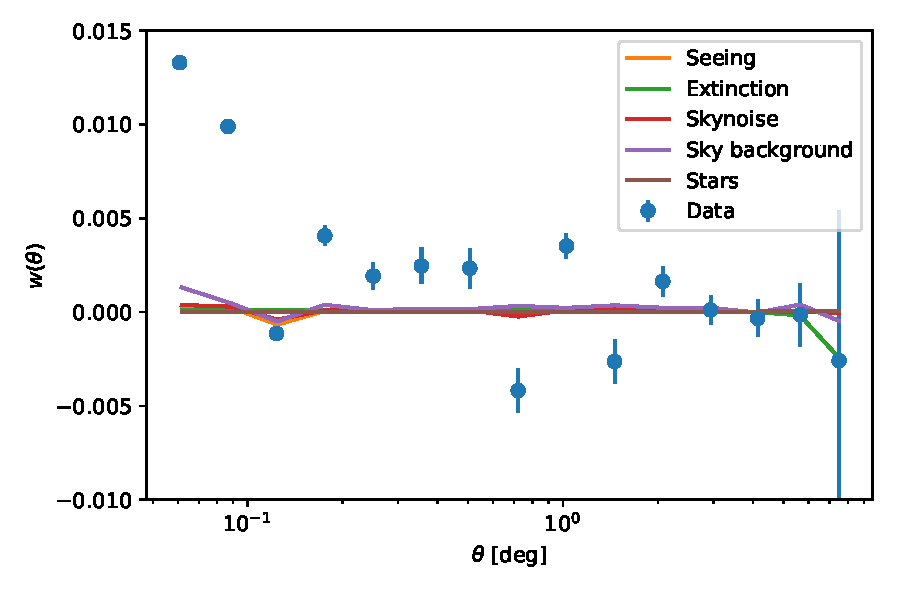
\includegraphics[width=0.9\columnwidth]{w_dithered_25p3.pdf}
%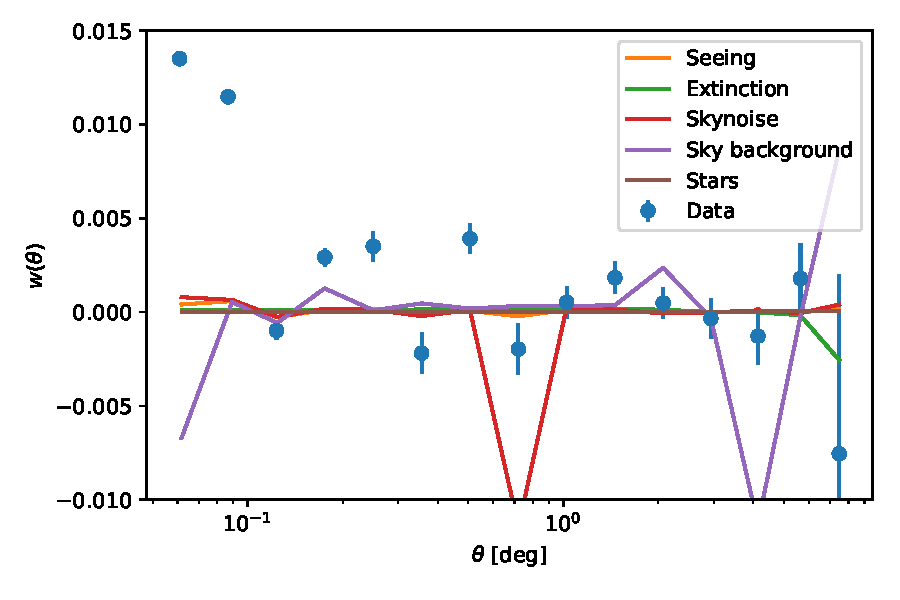
\includegraphics[width=0.9\columnwidth]{w_undithered_25p3.pdf}
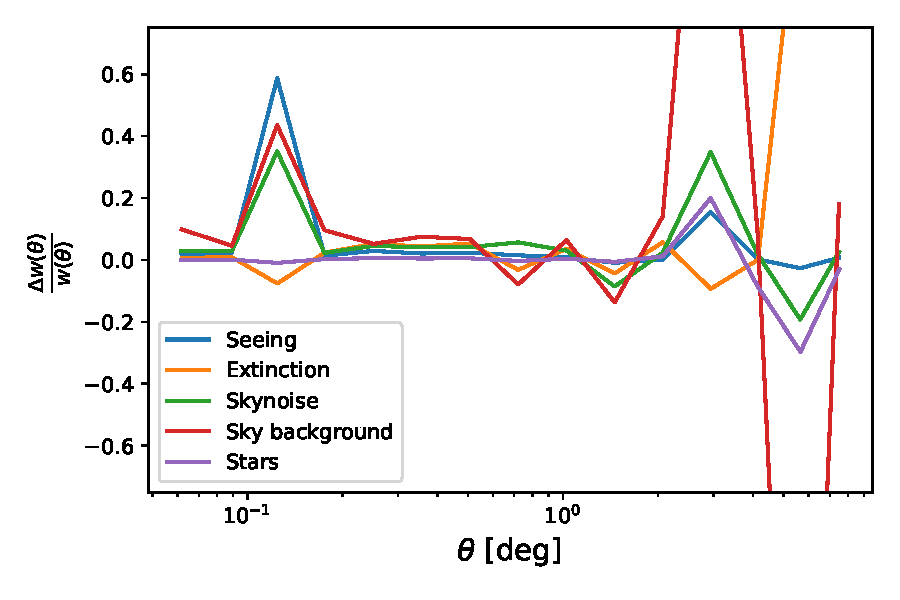
\includegraphics[width=0.9\columnwidth]{sys_dithered_25p3.pdf}
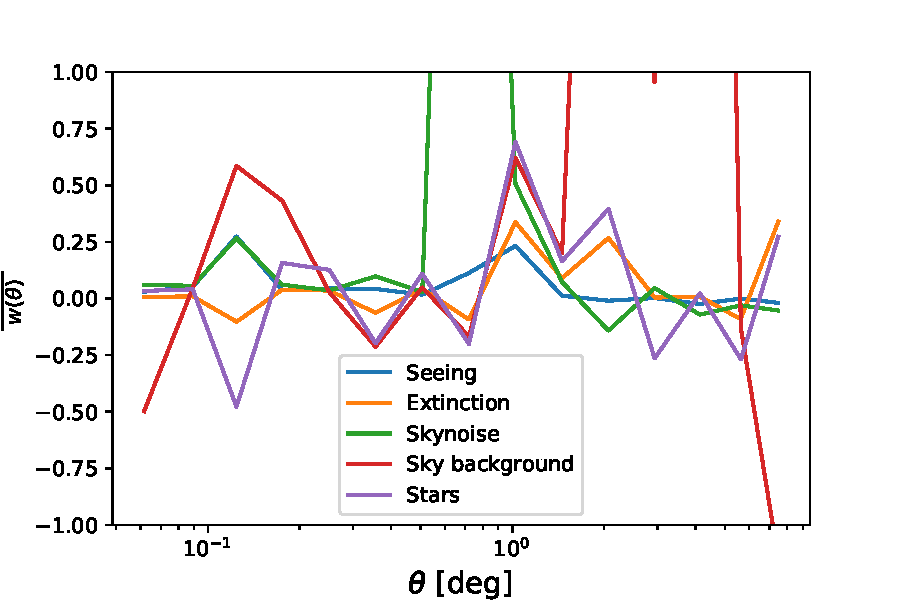
\includegraphics[width=0.9\columnwidth]{sys_undithered_25p3.pdf}
\caption{Correction due to the different potential sources of systematic uncertainty relative to the value of the measured correlation function of the dithered (top) and undithered (bottom) datasets.}
\label{fig:sys_realspace}
\end{figure}

\begin{figure}
\centering
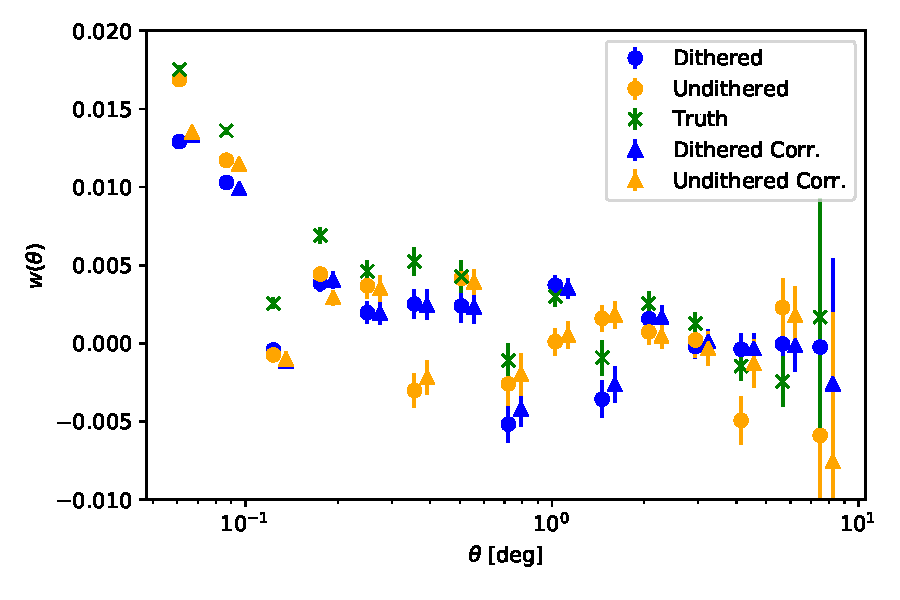
\includegraphics[width=0.9\columnwidth]{w_comp_corr25p3.pdf}
\caption{Results for the two-point correlation function in the input (green), dithered (blue) and undithered (orange) datasets. We can see that after the correction (triangles) for the systematic effects the agreement is better than without the correction (circles) between the input and output data especially for the undithered case (for the dithered case the corrections are negligible).} 
\label{fig:2pt_corr}
\end{figure}
\subsection{Pushing the dataset further}

% ----------------------------------------------------------------------

\section{Conclusions}
\label{sec:conclusions}

In this paper we presented the methodology to characterize the transfer function of LSST. This methodology can be easily exported to different photometric surveys. First, we performed a quality assessment of the data produced by the pipeline. Then, we generated the mask to perform our clustering analyses. Finally we compared the input and output two point clustering statistics to characterize the transfer function. \CHECK{Add more things when we have more results}.


% ----------------------------------------------------------------------

\subsection*{Acknowledgments}

Here is where you should add your specific acknowledgments, remembering that some standard thanks will be added via the \code{acknowledgments.tex} file.

%
The DESC acknowledges ongoing support from the Institut National de Physique Nucl\'eaire et de Physique des Particules in France; the Science \& Technology Facilities Council in the United Kingdom; and the Department of Energy, the National Science Foundation, and the LSST Corporation in the United States.  DESC uses resources of the IN2P3 Computing Center (CC-IN2P3--Lyon/Villeurbanne - France) funded by the Centre National de la Recherche Scientifique; the National Energy Research Scientific Computing Center, a DOE Office of Science User Facility supported by the Office of Science of the U.S.\ Department of Energy under Contract No.\ DE-AC02-05CH11231; STFC DiRAC HPC Facilities, funded by UK BIS National E-infrastructure capital grants; and the UK particle physics grid, supported by the GridPP Collaboration.  This work was performed in part under DOE Contract DE-AC02-76SF00515.
This manuscript has been authored by Fermi Research Alliance, LLC under Contract No. DE-AC02-07CH11359 with the U.S. Department of Energy, Office of Science, Office of High Energy Physics.

% 


%{\it Facilities:} \facility{LSST}

% Include both collaboration papers and external citations:
\bibliography{lsstdesc,main}

\appendix
\section{Mapping observational effects}
\label{sec:systematic_maps}
\begin{figure}
\centering
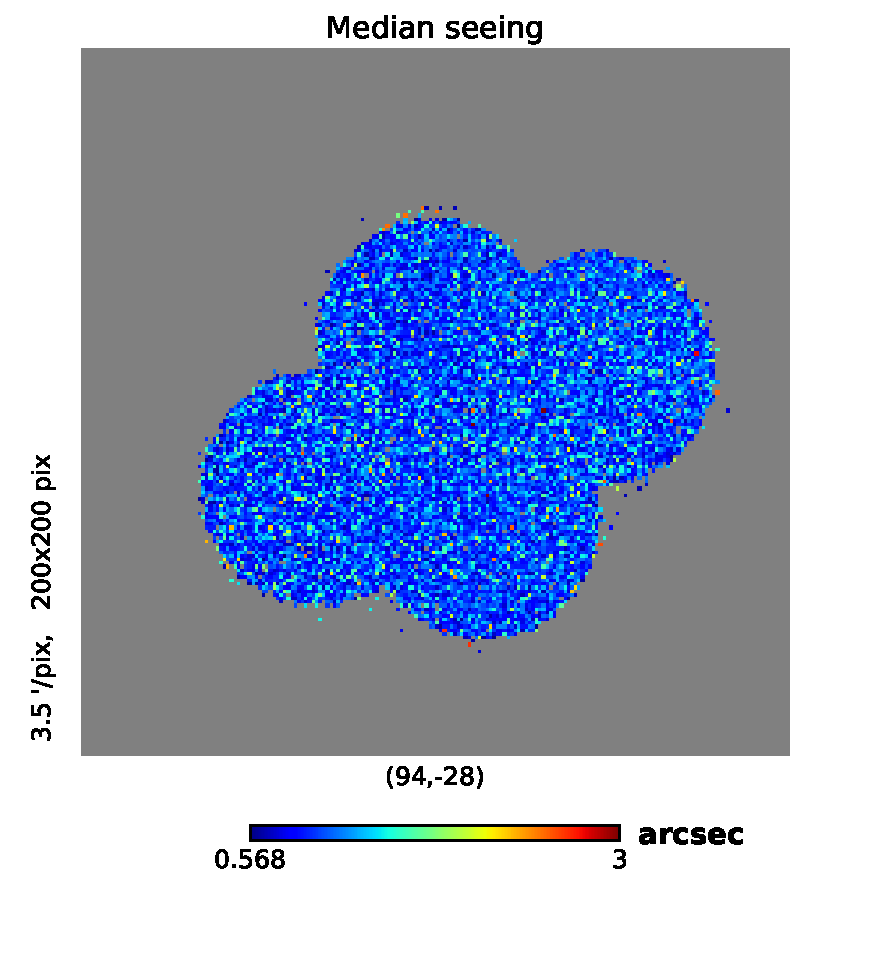
\includegraphics[width=0.9\columnwidth]{median_seeing_2048.pdf}
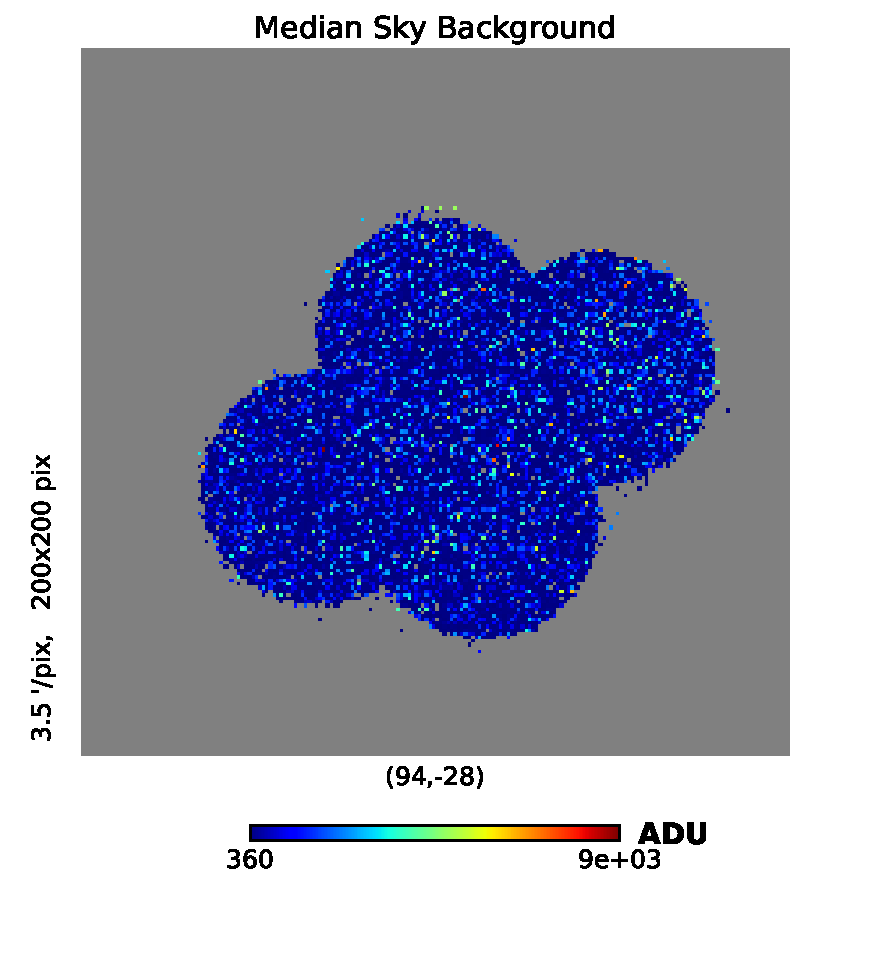
\includegraphics[width=0.9\columnwidth]{median_skybg_2048.pdf}
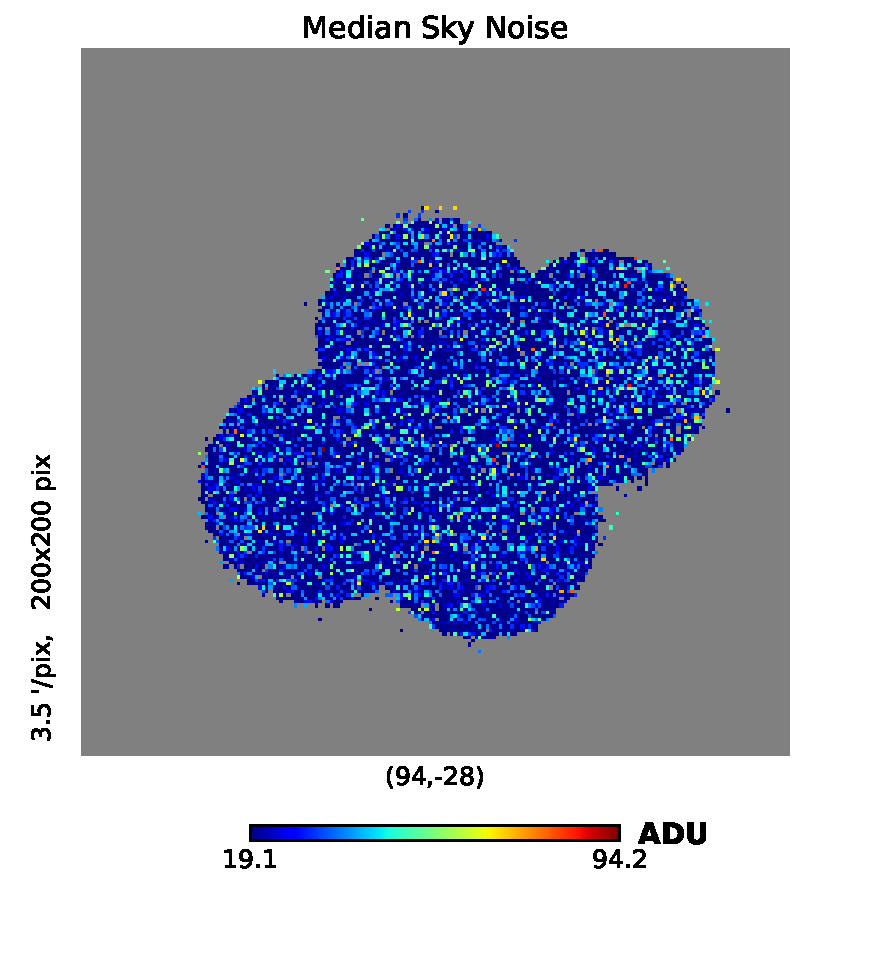
\includegraphics[width=0.9\columnwidth]{median_skynoise_2048.pdf}
\caption{HEALPix maps showing the different observational effects that might be potential cause of systematic uncertanties.}
\label{fig:systematic_maps}
\end{figure}
\begin{figure}
\centering
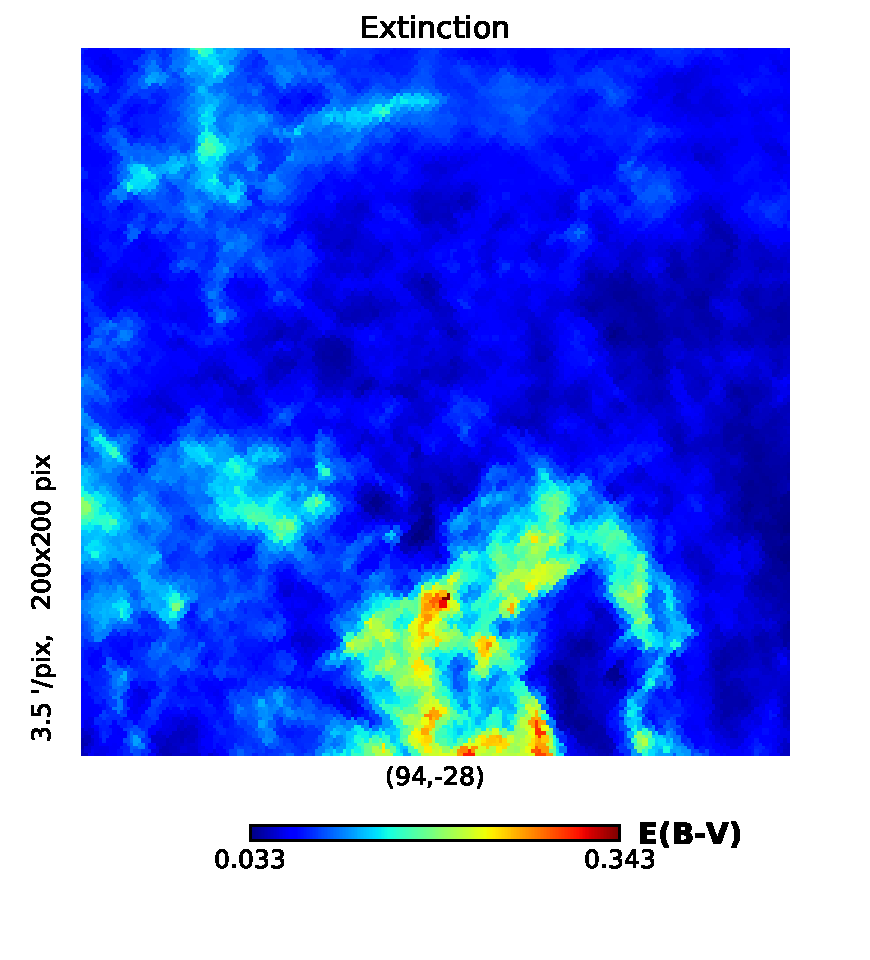
\includegraphics[width=0.9\columnwidth]{extinction_SFD.pdf}
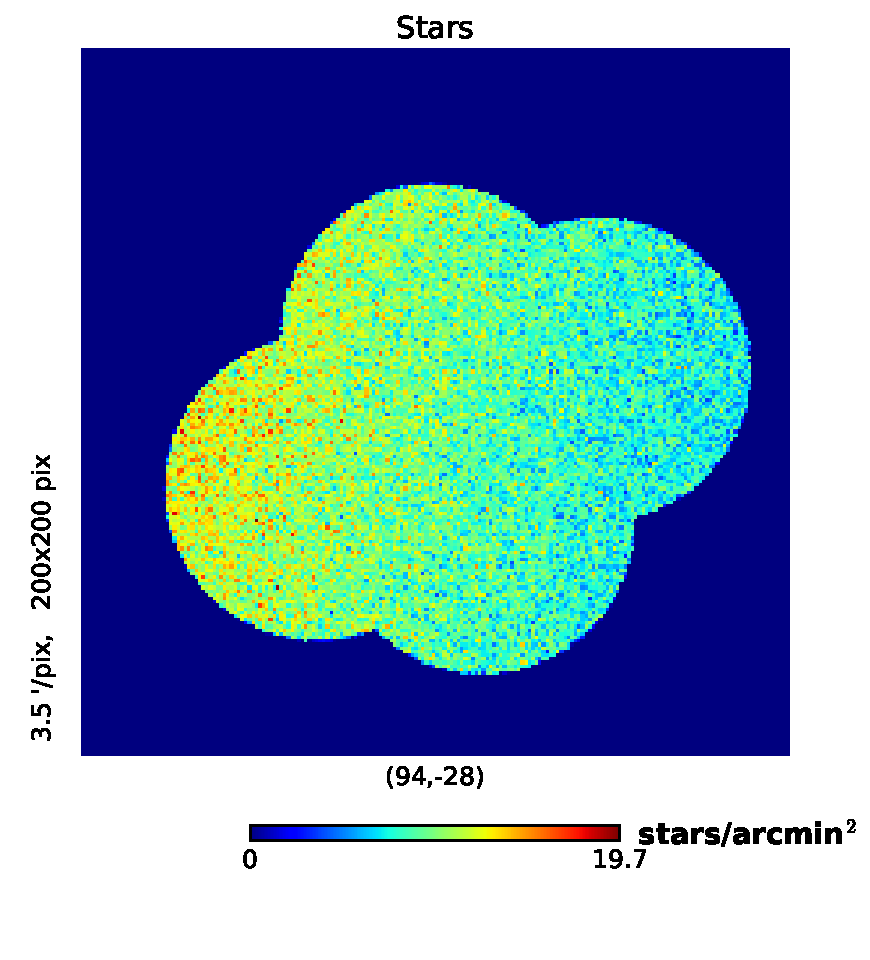
\includegraphics[width=0.9\columnwidth]{stars_map_2048.pdf}
\caption{HEALPix maps showing the different observational effects that might be potential cause of systematic uncertanties.}
\label{fig:systematic_maps2}
\end{figure}
\end{document}
% ======================================================================
%
